%!tikz editor 1.0
%!tikz source begin
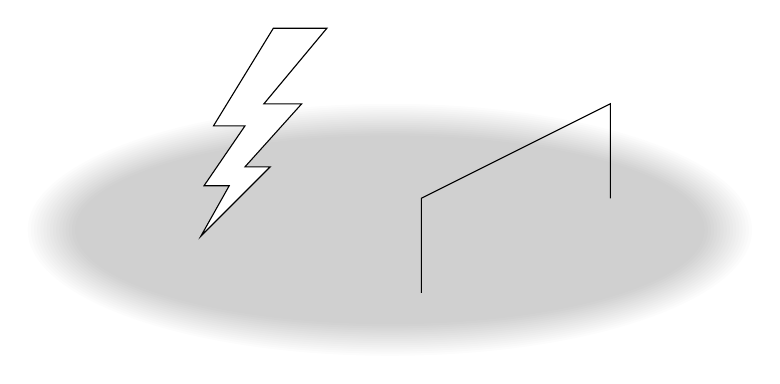
\begin{tikzpicture}[scale=0.8, transform shape]
%\fill [black, fill opacity = 0.075] (2,0.8) ellipse [x radius = 5, y radius = 1.5];

\foreach \i in {0,2,...,30}
        \fill [black, fill opacity = 1/100] (2,0.8)
          ellipse [x radius = 5+\i/40, y radius = 1.5+\i/60];

\fill [draw,fill=white] (1,4) to ++ (-1,-1.2) to ++ (0.6,0) to ++ (-0.9,-1) to ++ (0.4,0) to ++ (-1.1, -1.1) node (bot) {} to ++ (0.45,0.8) to ++ (-0.4,0) to ++ (0.65,0.95) to ++ (-0.5,0) to ++ (0.95,1.55) -- cycle;

\draw (bot) ++ (3.5,-0.9) to ++ (0,1.5) to ++(3,1.5) to ++ (0,-1.5);
\end{tikzpicture}
%!tikz source end
